\chapter{Introduction}
%intro st 1
Black Holes (BHs) are both extreme and ubiquitous objects which are increasingly becoming seen as unique laboratories to investigate gravity. The first inferences of their existence came from the observations of the highly energetic Active Galactic Nucleus (AGN) Cygnus~A as well as the rapid variability of quasars, both implying a massive and compact engine \citep[e.g.][and references therein]{Narayan_2013}. Since then, the case for accretion onto a BH powering highly energetic events such as kiloparsec-scale jets and gamma ray bursts have strengthened considerably, however the mechanisms by which these observables are produced are still under active debate. There are also unconstrained parameters regarding the nature of the event horizon and the surrounding space-time. The challenge in these investigations is robust imaging of the innermost black hole emission on sub-event horizon scales. However, this could change within the next few years as a novel observatory begins full operation.

\section{Unsolved questions in black hole astrophysics}\label{sec:unsolved_qs}
%st1
%The point is to give astrophysical meaning to the project

%plan 
We will now provide the astrophysical motivation for this thesis through a discussion of several key questions in black hole astrophysics which could be directly addressed through observations which resolve the innermost emission region. Later in this chapter we present an upcoming network of telescopes, observing at mm-wavelengths, which attempts to achieve this goal. 


%formation and mass classes 
BHs are formed through the gravitational collapse of a stellar core during a supernovae explosion or from direct collapse from a primordial gas cloud \citep[e.g.][]{Begelman_2006}. They can grow in mass through accretion of nearby material and/or mergers with other black holes. The observed BH mass distribution is separated into two distinct mass classes, stellar and supermassive - the former with mass on the order $M \sim 10 M_\odot$ and the latter $M \sim 10^6 - 10^{10} M_\odot$ \citep{Falcke_2013}. SMBHs form and reside (unless ejected) in the centres of all galaxies \citep{Kormendy_1995}. Observations of their surrounding galactic bulges show tight correlations between BH mass and both the bulge luminosity and stellar velocity dispersion \citep[e.g.][]{Magorrian_1998,Gebhardt_2000}, suggesting coevolution or feedback processes. 


%constraining event horizon scale physics 
To constrain the physics near a black hole, the observation needs to be sensitive to scales comparable to the event horizon. For a non-spinning (Schwarschild) black hole, the event horizon is spherically symmetric with a radius, 
\begin{equation}
R_{\rm Sch} = 2 R_{\rm G} = 2 {\rm G} M_{\rm BH} /{\rm c}^2,
\end{equation}
where $R_{\rm G}$ is the Gravitational radius, $M_{\rm BH}$ is the black hole mass, ${\rm G}$ is the gravitational constant and ${\rm c}$ is the speed of light. The angular size of such an event horizon in the far-field approximation is
\begin{align}
\theta_{\rm Sch} &= R_{\rm Sch} / d_{\rm src}\\
&\approx 0.02^{\prime \prime} \times 10^{-9} (M_{\rm BH}/M_\odot)({\rm kpc}/d_{\rm src}),
\end{align}
where $d_{\rm src}$ is the distance from observer to source. 

%SgrA is best candidate 
Due it's size and proximity, the BH with the largest $\theta_{\rm Sch}$ turns out to be the SMBH in the centre of our own galaxy, Sgr~A*. For Sgr~A$^\star$, optical/infrared monitoring of orbiting stars \citep{Gillessen_2009} has yielded ${M_{\rm BH} = 4.30 \pm 0.36 \times 10^{6} M_\odot}$ and ${d_{\rm src}= 8.28 \pm 0.32}$~kpc. Hence, for Sgr~A*,  $$\theta_{\rm Sch} \approx 10 \mu{\rm arcsec}.$$

\subsubsection{Innermost accretion and jet launch physics}
%st1

%Accretion + jet launch intro + motivation  and relativistic jets as a common feature.
The accretion of plasma onto compact objects is a fundamental process in astrophysics, occurring over many orders of magnitude of mass and accretion rate. Closely associated with accretion onto compact objects is the launch of highly energetic, relativistic jets which can remain collimated over large cosmological distances e.g. $\sim 120$~kpc for Cygnus~A \citep{Perley_1984}. In general, both accretion disks and jets are highly luminous sources of emission. The primary emission mechanism is synchrotron radiation (except at the highest energies where inverse-Compton dominates) which is radiated by relativistic electrons spiralling in a magnetic field. Key features of synchrotron emission is a broad power-law spectrum and strong linear polarisation. Self-absorption accompanies the emission and changes the shape of the spectral energy distribution as the optical depth of such a source is typically inversely proportional to the frequency. 
%for SgrA* st 1
The spectral energy distribution of Sgr~A$^\star$ peaks sharply in sub-millimetre, which for a self-absorbed synchrotron source implies that the emission becomes optically thin at these frequencies, and that the sub-millimetre emission arises from event horizon scales. \citep{Serabyn_1997,Falcke_1998}. 


%jet launch - generalised penrose
Theoretical studies and General Relativistic Magneto-Hydrodynamic (GRMHD) simulations of accreting SMBHs \citep[e.g.][]{Gammie_2003,Narayan_2012,Moscibrodzka_20133} have provided powerful demonstrations and arguments for how energy and angular momentum is transported in the system, including jet launch mechanisms. \citet{Penrose_1969} showed analytically that the rotational energy of a BH could provide the necessary power for jet formation. Associated GRMHD simulations (known as `generalised Penrose processes') typically start with a SMBH surrounded by a torus of gas threaded with a weak (compared to thermal energy) toroidal magnetic field. However, weakly magnetised disks are dynamically unstable if the angular momentum decreases with radius \citep{Balbus_1998}. This differential rotation provides the source of energy in the system as it forms the non-linear Magneto-Rotational Instability (MRI) which in turn creates turbulence in the geometrically thick disc. Through turbulence the gas loses angular momentum and gravitational energy, causing mass and magnetic field to be accreted nearer to the BH, in turn causing the inner region of the accretion flow to become highly magnetised. As the BH rotates, magnetic field lines get twisted up by the rotation of the plasma and space-time around BH, forming a strong poliodal magnetic  field. These ``helical magnetic springs'' \citep{Narayan_2014} expand, carrying with them, the threaded plasma along the poloidal field lines, resulting in jet launch.  



We will now briefly discuss two variants of the generalised Penrose process, which have physical applicability to SMBHs, Sgr~A* and M87.
 
%RIAF - sgrA
Radiatively Inefficient Accretion Flow \citep[(RIAF),][]{Narayan_1995,Yuan_2003} models offer a popular explanation for the observed ultra-low luminosity $\sim 10^{-8} L_{\rm edd}$ and accretion rate of Sgr~A*. The accretion rate is $\le 10^{-4}$ of the mean rate required to grow its mass withiin the Hubble time, despite the comparatively large amount of gas available for accretion within the Bondi radius \citep{Goddi_2016}. In the RIAF model the electron and proton temperatures decouple due to the low density of the gas. Most of the gravitational energy is converted into the viscous thermal energy of protons which radiate inefficiently compared to electrons. The protons are then either advected into the SMBH \citep{Narayan_1998} or ejected via outflows possibly in the form of winds or a low powered jet \citep{Blandford_1999}. 


%MAD - M87
In contrast, the powerful jet in M87 is thought to be powered by an accretion disc in the Magnetically Arrested Disc \citep[(MAD),][]{Narayan_2003} state, wherein mass accretion to the BH is suppressed by the strong magnetic field build-up near the black hole. Compared to Sgr~A*, M87 is on the other end of mass ($\sim 10^9 M_\odot$) and accretion rate ($\sim 10^{-4} L_{\rm edd}$) spectrum. The location of the jet base in M87 is in relation to its event horizon could help to constrain whether jet powered by the BH as opposed to the accretion disc.


%difficulties with grmhd sims and the need for observations
Hence theoretical and computational approaches are beginning to understand these processes, however the range of physical scales needed to be simulated, as well as uncertainties in the microphysics, make a theoretical approach difficult. Whether or not these processes are scale invariant, as suggested by the `fundamental plane of black hole activity' \citep{Merloni_2003}, remains to be determined and horizon scale observations are still needed to robustly compare models. Observations which can constrain the configuration of magnetic fields in the inner accretion/jet launch region are essential, and have already made an impact \citep{Johnson_2015b}.

\subsubsection{Measuring the black hole shadow}
%st1

%Lensing and the photon ring  
Fortunately, the innermost emission is gravitationally lensed by the SMBH, which causes it to appear magnified by several times its original angular size. In theory, the innermost orbit should be occupied by a ring of photons, the lensed image of which should feature a shadow-like (or `silhouette') feature \citep{Bardeen_1973,Luminet_1979, Falcke_2000,Takahashi_2004, Johannsen_2010}. Fig.~\ref{fig:grmhd} shows a cartoon illustration of the ray tracing combined with an early calculation of the ray-traced image of a thin accretion disc around a BH \citep{Luminet_1979}. The circular shadow is apparent as the silhouette of the lensed emission originating from the far side of the disc. 



\begin{figure}[h!]
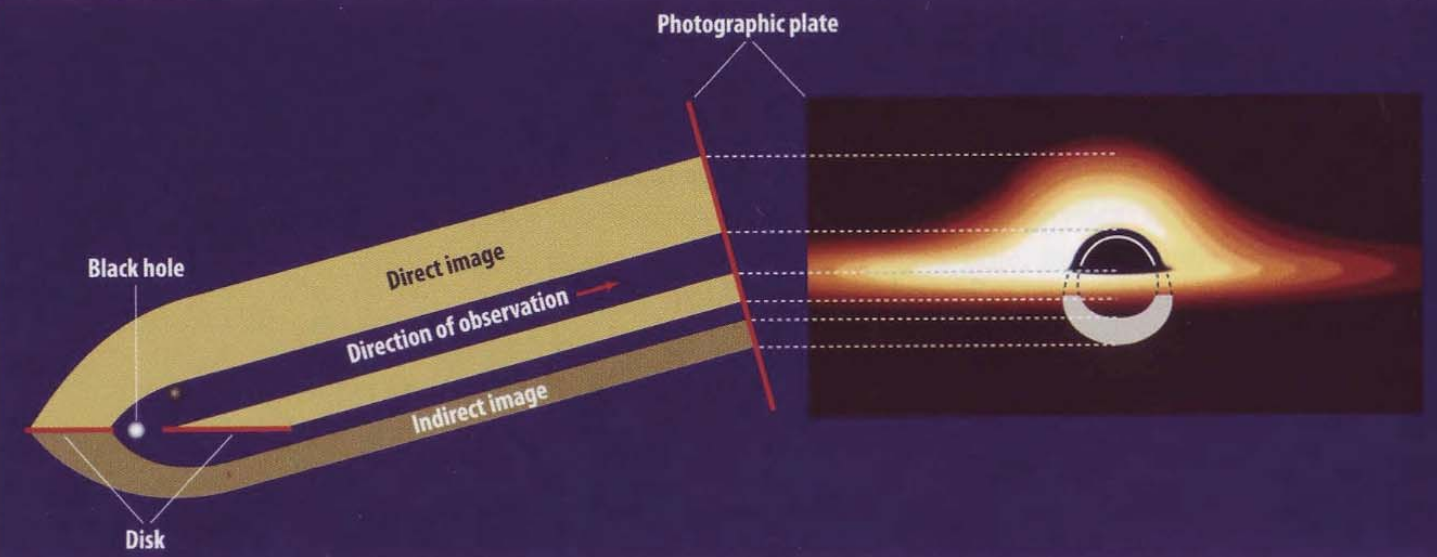
\includegraphics[width=\columnwidth]{Images/lensed_cartoon}
\caption{(Image credit : Shep Doeleman) Cartoon image (left) combined with the ray-tracing of a thin accretion disc surrounding a BH, first calculated by \citet{Luminet_1979}. The cartoon image shows that both the bottom and top of the far side of the accretion disc is lensed by the black hole and is superimposed on the image of the near side of the accretion disc. The dark area in the centre, known as the black hole shadow is the lensed image of the photon ring orbiting the BH. A measurement of its precise shape is a test of general relativity in the strong field regime. Note that the left-right asymmetry in the image is due to doppler boosting. \label{fig:grmhd}%
}
\end{figure}


%Probing strong gravity and black hole spacetime 
Gravity as described by General Relativity (GR) is consistent with all observational experiments thus far \citep[e.g.][and references therein]{Kramer_2006}, however GR has conceptual weaknesses, especially as it is not compatible with the quantum description of reality. Various alternatives to GR have been theorised which do not assume a purely classical description of matter. To compare GR with the alternatives, we have to compare its predictions in the strong, non-linear field regime where the largest deviations from GR would occur if it were an approximate theory.


The space-time within several $R_g$ around a SMBH provides such an opportunity. The precise shape of the photon ring around a SMBH is dependent on the space-time, which in turn is calculated within a theory of gravity \citep{Takahashi_2004}. The No-Hair theorem, which is based on GR, states that the space-time should only be determined by the first two moments of the black hole, i.e. it's mass and spin assuming no charge \citep[][and references therein]{Hawking_1972}. If the No-Hair theorem is invalid, the ring will deviate from a Schwarschild or Kerr profile. In the case of a non-zero quadrupole moment the ring will become either oblate or prolate \citep[e.g.][]{Johannsen_2010}. 

\section{The power of high angular resolution}
%st 1 
%Increasing resolution -> motivation and difficulties
Throughout the history of astronomy, there have been celestial sources which appear point-like (unresolved) with the available instrumentation. To investigate the nature of these sources, ever more sophisticated instruments with higher resolution are developed across the EM spectrum. 

In principle, a diffraction-limited aperture can obtain an angular resolution of
\begin{equation}\label{eq:ang_res}
 \theta_{\rm res}\ \approx \ 1.22\ \lambda / D {\rm rad},
\end{equation}
where $D$ is the diameter of the aperture and $\lambda$ is the observing wavelength. However, dish apertures larger than a hundred metres are infeasible or too costly to construct while systematic errors, including scattering-induced blurring due to inhomogeneous density (radio) or temperature (optical/NIR) distributions in the Earth's atmosphere can lead to instruments being unable to reach the diffraction limit. To overcome these difficulties and improve $\theta_{\rm res}$, a variety of new technologies have been developed (see Fig~\ref{fig:spec_ang}), including space-based observatories which escape the limitations set by the Earth's atmosphere; interferometric arrays which eliminate the need to build extremely large apertures; as well as technology-enabled mitigation strategies like adaptive optics and water vapour radiometry which account for atmospheric turbulence in real time. 


%Very Long Baseline Interferometry -> the highest resolution
The observing technique which typically achieves the highest angular resolution is Very Long Baseline Interferometry (VLBI). Interferometry refers to the technique of measuring the electric field correlations (named `visibilities') between pairs of separated antennae at suitably synchronised timing accuracy. The visibilities are related to Fourier components of the sky brightness distribution. Through an `adequate' sampling of the Fourier domain an approximate image of sky can be reconstructed using the inverse Fourier transform. With this method, the distance between the antennae ($\bm{b}$, referred to as the `baseline') effectively replaces $D$ in equation~\ref{eq:ang_res}, yielding higher angular resolution than a single aperture. This technique is primarily used at radio frequencies while the electric field phase remains relatively stable. VLBI is essentially radio interferometry with antennae separated by large distances, typically $\gtrsim 100$~km, including the possibility for antennae in Earth's orbit. A key distinction from connected-element interferometery is that independent clocks are needed at each station to facilitate the post-observation correlation. VLBI has seen several noteworthy achievements since its inception in the late 1960's. This includes the resolution of quasars into core-jet systems and the appearance of super-luminal motion of the jet components \citep[e.g.][]{Whitney_1971}, the mapping of maser motion around the Super-Massive Black Holes (SMBH) in the cores of nearby galaxies \citep[e.g.][]{Miyoshi_1995} and the resolution of expanding supernovae shells \citep[e.g.][]{Pedlar_199}.


%fig : angular resolution across spectrum
\begin{figure}[h!]
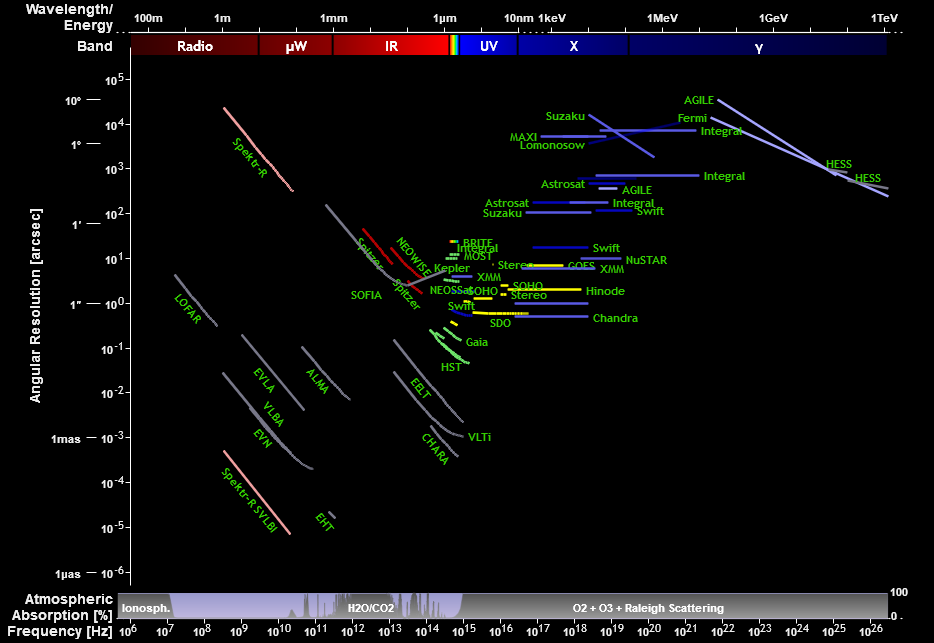
\includegraphics[width=\columnwidth]{Images/spec_ang}
\caption[An illustration of angular resolution vs. observing frequency across the entire observational spectrum, shown for a selection of observatories. The VLBI arrays : Spektr-R SVLBI (or RadioAstron) and the EHT clearly achieve the highest angular resolution of all due to their long baselines.]{(Image credit: Olaf Frohn\protect\footnotemark[1]) An illustration of angular resolution vs. observing frequency across the entire observational spectrum, shown for a selection of observatories. The VLBI arrays : Spektr-R SVLBI (or RadioAstron) and the EHT clearly achieve the highest angular resolution of all due to their long baselines. At the bottom of the plot, there is a panel showing atmospheric/ionospheric absorption as a function of wavelength, and consequently all observatories in the zero transmission zones are space-based. \label{fig:spec_ang}
}
\end{figure}
\section{The Event Horizon Telescope}
%st 1

\subsubsection{Overview}
% EHT -> intro to the Array st 1
In the last few decades there has been a push to enhance VLBI capabilities at sub-millimetre wavelengths. One of the leading efforts in this regard is the Event Horizon Telescope consortium \citep[(EHT),][]{Doeleman_2010}, an international project whose primary objective is to spatially resolve the lensed photon rings of nearby SMBHs with an angular resolution on the order of their event horizons. In contrast to other high frequency VLBI networks, which have a maximum frequency of 43~GHz (7~mm) or 87~GHz (3.5~mm), the EHT is operating at 230~GHz (1.3~mm) and will potentially extend up to 345~GHz (0.8~mm) in the future. See Fig.~\ref{fig:eht_globe} for an annotated map of the locations of the EHT array. As the EHT has baseline lengths comparable to the diameter of the earth, $|b| \sim 10^4$~km and is operating at 1.3~mm, this yields $\theta_{\rm res} \sim 30\ \mu$-arcsec.  The two primary targets Sgr~A$^\star$ and M87 are expected to have gravitationally-lensed photon rings with apparent angular diameters of $\theta_{\rm pr} \sim 50$ and $\sim 20-40\ \mu$-arcsec respectively \citep*{Falcke_2013, Broderick_2009}, and hence should be resolvable by the EHT. 
\footnotetext[1]{http://armchairastronautics.blogspot.co.za/p/space-observatories.html}

\begin{figure}[h!]
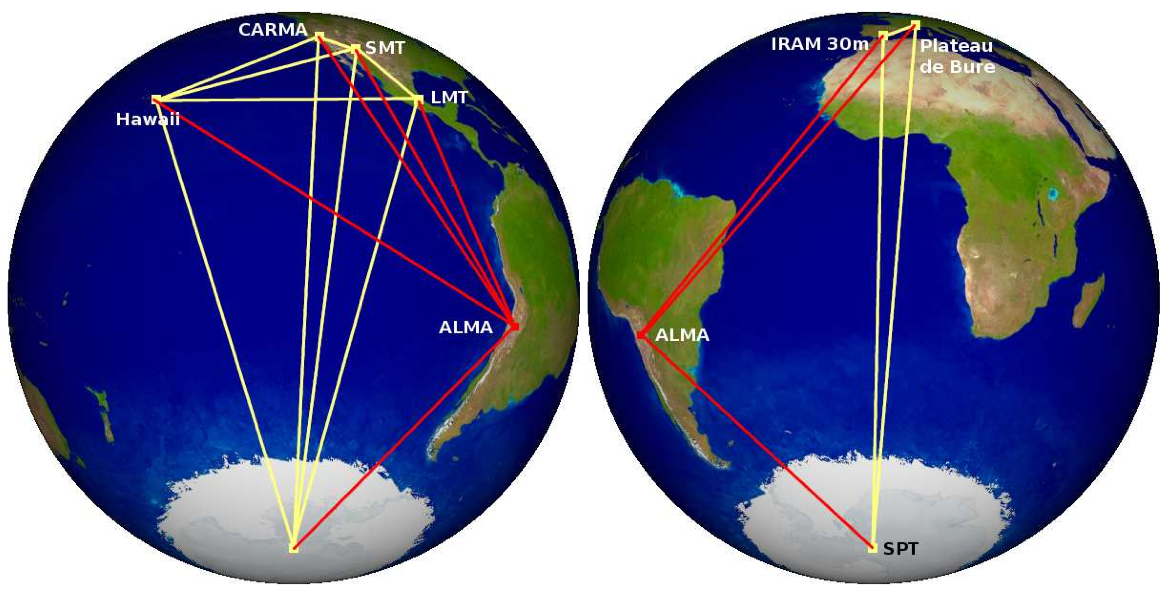
\includegraphics[width=0.8\columnwidth]{Images/eht_globe}
\caption{(Image credit: Remo Tilanus) The view of the Event Horizon Telescope (EHT) from Sgr~A*. This interferometric array uses Earth-diameter baselines, operating at $230-345$~GHz to attain an angular resolution of the order of ${\theta_{\rm res} \sim 10\ \mu}$-arcsec. Baselines to ALMA are shown in red, to highlight its order of magnitude higher sensitivity. Note that the CARMA station has recently been decommissioned, a telescope in Greenland is currently being constructed and there is ongoing investigation into a possible site on the African continent.\label{fig:eht_globe}%
}
\end{figure}



\subsubsection{Instrumentation and observational challenges}\label{sec:eht_obs}

%intro - newness of field and instrument st 1
The development of mm-VLBI instrumentation has been spurred by the formation of EHT as a project and the deepening of theory and simulation work over the past two decades. This is evidenced by the comparable observational results but starkly different interpretations of \citet{Krichbaum_1998} and \citet{Doeleman_2008}. A decade apart, both teams observed Sgr~A* with a mm-VLBI arrays consisting of three stations at similar frequency (215~GHz in 1998 and 230~GHz in 2008). Although the former was limited by calibration uncertainties, the primary difference in analysis and interpretation was that the latter result was linked explicitly to the innermost accretion physics in the event horizon region \citep[e.g.][]{Broderick_2011}. In this way, the newly developed theoretical context contributed to the significance of the \citet{Doeleman_2008} result. However, a robust comparison with this diverse body of theoretical work would require a significant leap in mm-VLBI observational capabilities. For example, to discern whether the No-Hair theorem is violated requires the fractional asymmetry of the shadow shape with respect to its angular size to be measured to a few percent \citep[e.g.][and references therein]{Goddi_2016}. To achieve this level of precision, the development of the global mm-VLBI array will face significant challenges.


%moving to higher freq st 1
The move to higher frequencies is accompanied by requirements on the instrument including: increased data rates ($1 \to 16$~GHz) and stability of timing standards; as well as increased accuracy of dish surfaces and antenna pointing accuracy. Difficulties emerge also from the effects of the Earth's lower atmosphere where optical depth becomes significant and turbulence causes rapid fluctuations in the signal transmission time which causes decoherence in the visibilities. Even though the stations are at high altitude, desert locations, the atmospheric coherence times are still short, typically $\lesssim$10~s \citep{Doeleman_2009}. The extensive requirements on instruments and location drive up the cost of mm-VLBI stations, resulting in few element ($<10$) interferometric arrays which make for sparse sampling of the Fourier domain. This is exacerbated by short mutual visibility windows and imperfect weather. Traditional phase referencing calibration is ruled out due to the variable atmosphere, the low sub-mm source density and that calibrators are resolved and variable too at this high angular resolution. 


%More complicated effects 
Aside from the considerations listed above, there is a string of complications relating to the sources, the ISM and the calibration procedure. 
%ISM st 1
Firstly the emission from the primary source, Sgr~A*, is strongly scattered by a turbulent electron plasma in the Interstellar Medium (ISM) along the line-of-sight to the Galactic Centre. This results in a blurring effect \citep[e.g.][]{Fish_2014} which falls as $\nu^{-2}$ and become sub-dominant to intrinsic structure in the sub-millimetre range, as shown in Fig.~\ref{fig:scattering_law}. This medium both blurs and introduces random, time-variable substructure into the source brightness distribution (see section~\ref{sec:ism_scat}). The scattering substructure adds complications for data interpretation as its contribution is difficult to disentangle from that of the intrinsic source substructure, depending on the time-scale of the observation.
%src variability
The second issue is that the source is intrinsically variable over minutes to hours (see section~\ref{sec:variability}). The fact that the source is variable over the course of a single observation epoch breaks a fundamental assumption in interferometry as the visibilities cannot be related to a static sky image. This (broken) assumption is central to technique of self-calibration and fringe-fitting (see section~\ref{sec:self_cal}).
%the intermingling
These signal corruptions and invalid assumptions appear to interlink in various ways which could generate subtle systematic errors in data analysis. 


% Effect of corruptions on Science extraction : parameter estimation and imaging, #HighAccuracy 
\begin{quotation}
``These effects, among others, may place significant limitations on the sensitivity, image fidelity, and dynamic range that can be achieved with mm-VLBI observations.  Furthermore, unaccounted for systematic and/or non-Gaussian uncertainties could preclude robust, accurate Bayesian parameter estimation and model selection analyses of accretion flow \citep[e.g.][]{Broderick_2016} and gravitational physics \citep[e.g.][]{Broderick_2014, Psaltis_2016}, two of the EHT's many objectives.''\\
\citep{Blecher_2016}
\end{quotation}


This point being made is that the data product used in the Bayesian parameter estimation routine, cannot be assumed to have only known Gaussian errors if the calibration procedure did not propagate the full Posterior Probability Distribution (PDF). Thus emerges the imperative for a quantitative understanding of mm-VLBI's ability to measure and discern between theoretical predictions in the presence of a myriad of signal corruptions.

\section{A realistic mm-VLBI simulator}
%St : 1

%Why simulate: intro 
Given the significant observational challenges that the EHT faces, we have undertaken this project to build a mm-VLBI observation and signal corruption simulator. There are many benefits for using such a toolkit and indeed synthetic data simulation is common practice for major scientific experiments. A prominent example is the extensive gravitational wave template matching scheme for The Laser Interferometer Gravitational-Wave Observatory (LIGO) which operates in the presence of tidal loading, passing trains etc. In essence such a simulator would fill in the final component of the theoretical signal propagation chain, effectively taking astrophysical simulations of the source (e.g. accretion onto a SMBH) as an input and returning realistic synthetic interferometric data. This allows a more effective interplay between theory and observation, quantifying systematic effects and the measurement limits. The remainder of this section will briefly discuss several research questions relevant to an EHT synthetic data simulator and how we approach the software design in order to address these questions. 

%Specific use cases of simulations

%Testing calim through standard challenges 
A key use case for simulated data is the testing of calibration, parameter estimation and imaging algorithms and strategies. As the inputs to the simulator are known exactly, we are better able to explore sources of error which are difficult to disentangle from intrinsic source features when using only real data. A straightforward way to perform such a test is through the creation of a set of `standard challenge' dataset. Such datasets would be available to the entire community to input into their calibration and/or imaging routines. Following this, a detailed comparison between the different strategies in varying regimes (source, ISM, troposphere and instrumental) can be made. Importantly, a systematic investigation of a particular algorithm across many different datasets could provide insight into subtle or previously unknowns sources of error inherent in that routine.


%Optimising observations 
Simulated data can also assist in the optimisation of the experimental configuration. Financial constraints require the prioritisation of hardware upgrades e.g. increasing bandwidth, surface accuracy improvement, deployment of water vapour radiometers or additional receiver bands. Simulated data together with calibration and imaging pipelines can help to quantify the benefit of each improvement based on expected scientific return in units of precision of the scientific parameter of interest (e.g. shadow assymetry) rather than more generic terms (e.g. angular resolution, positional uncertainty) that may not have an associated systematic effect included. This approach can even be extended to assess new candidate stations, especially as new geographic locations (e.g. in Southern Africa) are receiving increasing attention due to the potential long baselines to ALMA, SPT and European stations.


\begin{quotation}
%the Meqtrees+MS approach
``Over the past decade, significant effort has been placed on advanced radio interferometric calibration and imaging algorithms for centimetre and metre-wave facilities in response to the large number of new arrays in construction or design phase, including MeerKAT, Australian Square Kilometre Array Pathfinder (ASKAP), Square Kilometre Array (SKA), Low-Frequency Array (LOFAR), and the Hydrogen Epoch of Reionization Array (HERA). A leading software package in this pursuit is \textsc{MeqTrees}\footnote{https://ska-sa.github.io/meqtrees/} \citep*{Noordam_2010}, which was developed to simulate, understand and address the calibration issues to be faced with the greatly enhanced sensitivity, instantaneous bandwidth, and field-of-view of such facilities. \textsc{MeqTrees} is rooted in the Measurement Equation mathematical formalism \citep{Hamaker_1996}, which parametrises the signal path into distinct $2 \times 2$ complex  matrices called Jones matrices. This formalism and applications thereof are laid out in \citep{Smirnov_2011a,Smirnov_2011b,Smirnov_2011c} and are arbitrarily generalized to model any (linear) effect, including undesired signal corruptions that often may have subtle, yet systematic effects. \textsc{MeqTrees} has been applied to correct for direction dependent calibration errors to Karl. G. Jansky Very Large Array (VLA) and Westerbork Synthesis Radio Telescope (WSRT) observations, achieving record-breaking high dynamic range images \citep[][Makhathini et al, in prep.]{Smirnov_2011c}. The effectiveness provided by the Measurement Equation formalism in radio interferometric calibration provides a strong motivation to explore its application to the challenging goal of imaging a supermassive black hole silhouette with mm-VLBI.


%other simulation efforts 
Recently, there has been an increase in the attention given to simulating EHT observations of Sgr~A*  and M87 \citep{Fish_2014,Lu_2014,Bouman_2015,Lu_2016,Chael_2016}. However, these are primarily focused on image reconstruction and assume either negligible or Gaussian distributed gain errors; perfect antenna pointing accuracy; and in most cases only Gaussian convolution to simulate ISM scattering. Clearly, as the EHT array is enhanced (and possibly expanded), so too must the interferometric simulations evolve to provide ever-more physical predictions on the confidence levels with which parameters can be extracted and hence exclude theoretical models of gravity and/or accretion flows.


Given the significant, yet surmountable, observational challenges that the EHT faces, we have undertaken a project to leverage metre and cm-wavelength simulation and calibration successes and build a \textsc{MeqTrees}-based mm-VLBI-specific software package called \textsc{meqsilhouette}. While \textsc{MeqTrees} has not yet been used in the context of mm-wavelength observations, the framework is agnostic to higher frequency implementation as long as the Measurement Equation is appropriately constructed. \textsc{meqsilhouette} enables realistic interferometric simulations of mm-VLBI observations in order to gain deeper understanding of a wide range of signal propagation and calibration effects.''\\
\citep{Blecher_2016}
\end{quotation}
 
\section{Outline}
%st 1
This thesis is divided into the following chapters and sections,
\begin{itemize}
 \item {\bf Chapter 2 : Theory} 
 \begin{description}
  \item [Section 2.1] introduces radio interferometry via the Measurement Equation formalism, followed by mm-VLBI tailored discussions on calibration, data products and the consequences of breaking the static source assumption.
  \item [Section 2.2] is a review and investigation into the key signal corruptions implemented in the {\sc meqsilhouette} simulator i.e. instrumentation imperfections and transmission through the ISM and Earth's atmosphere.
 \end{description}

 \item {\bf Chapter 3 : Software Implementation}
 \begin{description}
  \item [Section 3.1] summarises the key software design objectives considered.
  \item [Section 3.2] is a description of the design and construction of the simulation software with emphasis on the software architechure and workflow.
 \end{description}

 
 \item {\bf Chapter 4 : Results}
 \begin{description}
  \item  [Section 4.1] showcases the basics of the simulator output through a series of canonical results.
  \item [Section 4.2] presents a more sophisticated scenario which tests an {\sc aips} calibration routine in the presence of source and tropospheric time-variability.
 \end{description}
 
  \item {\bf Chapter 5 : Discussion}
  \begin{description}
   \item [Section 5.1] explores the implications of the results shown in the previous chapter.
   \item [Section 5.2] makes suggestions for future applications of and improvements to the simulator.
  \end{description}

  
 
  \item {\bf Chapter 6 : Conclusions }\\
  We summarise the work and context of this thesis. 
\end{itemize}
















